\documentclass[dissertation.tex]{subfiles}

%TC:group code 0 0
%TC:group figure 0 0
%TC:macrocount \UoC 4
%TC:macrocount \mifare 1
%TC: macrocount \crypto 1
\begin{document}
  \chapter{Evaluation}

  % Overview paragraph about chapter
  % evaluation against goals and also performance analysis
  % particular decision

  The original aim of the project, as outlined in the proposal, was to develop a high-level \mifare{} library, a \mifare{} digital signature library, and a revocation gossip protocol for distributing revoked UIDs. The end result both encompasses the original goals, and additionally includes a simulation suite for simulating arbitrary networks of readers and cards. Whilst fulfilling the success criteria, the project has broadened slightly in scope, including additional countermeasures such as key diversification and emulated card detection, that further enhance security.

  \section{\mifare{} Library}
  Development of the \mifare{} library followed software-engineering best practices such as source code management (git) and comprehensive test coverage. The unit tests enabled me to catch several subtle mistakes which would have led to difficult to track down bugs, including one in a third party library. The library is structured to support future additions without breaking backwards compatibility. This would allow, for example, someone to easily add support for \mifare{} Desfire cards.

  The abstraction of the reader and card interfaces from their implementations was not only instrumental to the success of this project, but will also be of use to others writing software for interacting with \mifare{} Classic cards. Any software written on top of the library can benefit from the mock driver to write automated unit tests rather than relying on human and hardware based verification. The library will be open sourced and thus constitutes a significant contribution to the community.

  \subsection{Choice of Language}
  Go proved to be an excellent choice of language to implement the library in. Making the library cross-platform has required no effort on my part and the standard library that Go provides has been very useful, in particular its cryptographic packages and test framework.

  One of the original motivating factors behind the choice to use Go was its concurrency primitives and how they could be useful with the asynchronous nature of NFC communication. Whilst at a low level the communication with a card is asynchronous, I realised that it doesn't make sense to expose this in the library's API.\@ The concurrency primitives were utilised in the simulation suite and enabled a significant speedup of the CPU-bound simulations by running them in parallel.


  \section{Digital Signature Protection}

  The digital signature library is built on top of the \mifare{} library and uses the provided mock driver in its unit tests. The library provides methods for provisioning a signature, reading signed data, and writing signed data.

  To both verify that the library worked and serve as a demo, I wrote a small command line application for interacting with some physical \mifare{} 4K cards. The application simply stores and retrieves a username, it has three commands:

  \begin{itemize}
    \item \texttt{provision [username]} \\
      Allocates a sector for the username and a sector for the signature if not already allocated and writes the specified username.
    \item \texttt{sign} \\
      Signs the username and UID.\@
    \item \texttt{read} \\
      Reads the username and specifies whether the signature was valid.
  \end{itemize}

  The listing below shows the output when provisioning a new card. The signature is only valid after signing the username and UID.\@

  \begin{code}[numbers=none,gobble=0]{{}}
    $ ./demo/digsig provision alice
    Provisioning card with UID: 50492583
    Card provisioned

    $ ./demo/digsig read
    Name: alice [invalid]

    $ ./demo/digsig sign

    $ ./demo/digsig read
    Name: alice [valid]
  \end{code}

  The commands below use the \mifare{} offline cracker\footnote{\url{https://github.com/nfc-tools/mfoc}} to extract the secret keys from Alice's card and dump the data. The dump is then written to a different card. As this card has a different UID the signature is not valid.
  \begin{code}[numbers=none,gobble=0]{{}}
    $ mfoc -O alice.mfd
    ...
    $ nfc-mfclassic w B alice.mfd demo.mfd
    $ ./demo/digsig read
    Name: alice [invalid]
    $
  \end{code}


  \section{Ability to Mitigate Attack}

  It was never the aim of this project to completely ``secure'' \mifare{} Classic cards. The security of the cards is fundamentally compromised. As is concluded in prior research\cite{garcia2008dismantling} new deployments of NFC cards should use one of the several more secure alternatives such as the \mifare{} DESFIRE EV2.\@

  Organisations with existing deployments of \mifare{} Classic cards should still plan to upgrade to a more secure card. The process of upgrading a large deployment such as the one at \UoC{} is a complex and costly one, both financially and in terms of time. All readers would have to be upgraded to support the new type of card before any cards can be issued. At \UoC{} this includes readers belonging to several distinct departments and colleges, each of which has a different system.

  Until an NFC deployment can be upgraded or whilst it is ongoing, the countermeasures outlined in this project significantly enhance security. Without these countermeasures, an attacker need not have any technical expertise to mount an attack as software for cracking the cards is freely available. With the ease in which a malicious actor can access the tools required it would be surprising if the vulnerabilities weren't being actively exploited.

  \subsection{Impact on Attacks}

  \subsubsection{Forge a card}
  With knowledge of the structure of the data on one card an attacker can produce a different card. For example, at the University of Cambridge an attacker can create a new card with an arbitrary CRSID.\@

  Without the countermeasures there is no protection against this.

  With the digital signature countermeasure an attacker would need to also forge the signature and therefore this attack is prevented.

  \subsubsection{Clone a card}
  With access to a card an attacker can make a copy of the card.

  Without the countermeasures an attacker can extract the secret keys using freely available open source tools. This then allows them to clone any card to a blank card.


  The key diversification countermeasure means an attack must extract the secret keys from every card they wish to clone which takes several minutes. With the digital signature countermeasure an attacker must either have a card that allows the UID to be written or have specialist equipment that can emulate the \mifare{} Classic card. The emulation detection countermeasure additionally requires that any specialist equipment implement the same PRNG as the \mifare{} card to avoid detection. Even after this, a cloned card may be detected as the decrement counter will get out of sync.

  \subsubsection{Use a stolen card}
  Without the countermeasures the card will stop working with networked readers when it is reported stolen. The card will continue to work with offline readers unless they are manually updated.

  With the countermeasures the card will stop working with networked readers when it is reported stolen. The revocation gossip protocol will also  distribute the UID to the offline readers to prevent use with them after a short period of time.


  The key diversification countermeasure prevents an attacker using the secret keys from one card to access data on another, thus an attacker is required to have prolonged access to a card to access the data.

  \section{Applicability to Other Cards}
  Whilst the focus of this project was on \mifare{} Classic cards, it is far from irrelevant to other NFC cards. Many of the countermeasures outlined, such as digital signatures and the revocation gossip protocol are not inherently specific to \mifare{} Classic cards. The use of digital signatures with other NFC cards would provide \emph{defence in depth} --- a well accepted security principle in which security measures are layered upon each other to provide redundancy when one security measure fails.

  The revocation gossip protocol would be useful in any deployment with offline readers. The protocol could be altered to distribute other data such as reader configuration, allowing an organisation to update the configuration of offline readers.

  \section{Revocation Gossip Protocol}
  The goal of the revocation gossip protocol was to distribute the list of revoked card UIDs from online readers to offline readers. This allows an organisation to more effectively block the use of lost or stolen cards.

  The simulation suite supports simulating a wide range of different network layouts. It was used throughout the development of the gossip protocol to identify performance issues and inform changes to the algorithm. In this section, the performance of the revocation gossip protocol is assessed against a range of different simulations.

  \subsection{Best-case performance}

  If just a single UID is revoked, then every card that is tapped on an online reader will contain the UID in its revocation sector. Each of the algorithms is optimal in this case, and thus it serves as a useful baseline for the inherent difficulty of a particular network of readers.

  The simulation records the number of cards that tapped on each offline reader before the revoked UID was propagated to it. Figure~\vref{fig:sim_single_500} shows the best-case performance on a semi-randomised network (see Section~\ref{sec:topology}) consisting of 500 offline readers and 100 online readers. The graph plots the 50th, 90th, and 99th percentile of card taps for varying numbers of cards per reader.

  \begin{figure}[h]
    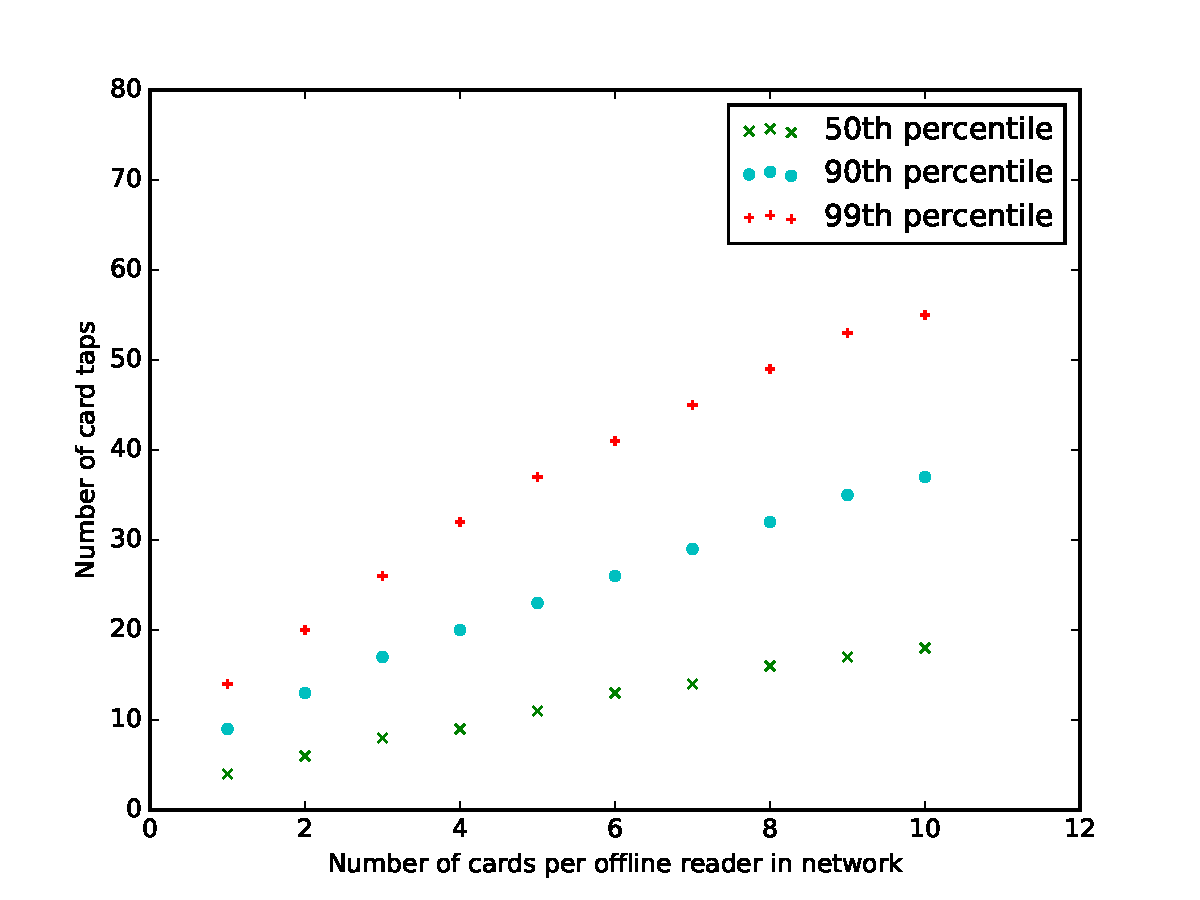
\includegraphics[width=\linewidth]{single_card_500.pdf}
    \caption{Card taps to update readers with revoked UID (\SI{500}{readers})}\label{fig:sim_single_500}
  \end{figure}

  It can be seen that as the number of cards increases, it takes more taps on average to propagate the UID to each reader. With 500 cards (one per offline reader), $99\%$ of readers are updated in 14 taps or less. With 5000 cards (ten per offline reader), $99\%$ of readers are updated in 55 taps or less.

  From first glance it may seem that the best case performance is negatively impacted by increasing the number of cards. This is, however, not the case, as increasing the number of cards also increases the frequency of card taps on a reader. Figure~\ref{fig:sim_single_500_time} shows that increasing the number of cards decreases the number of simulation timesteps required to propagate the UID.\@

  \begin{figure}[h]
    \centering
    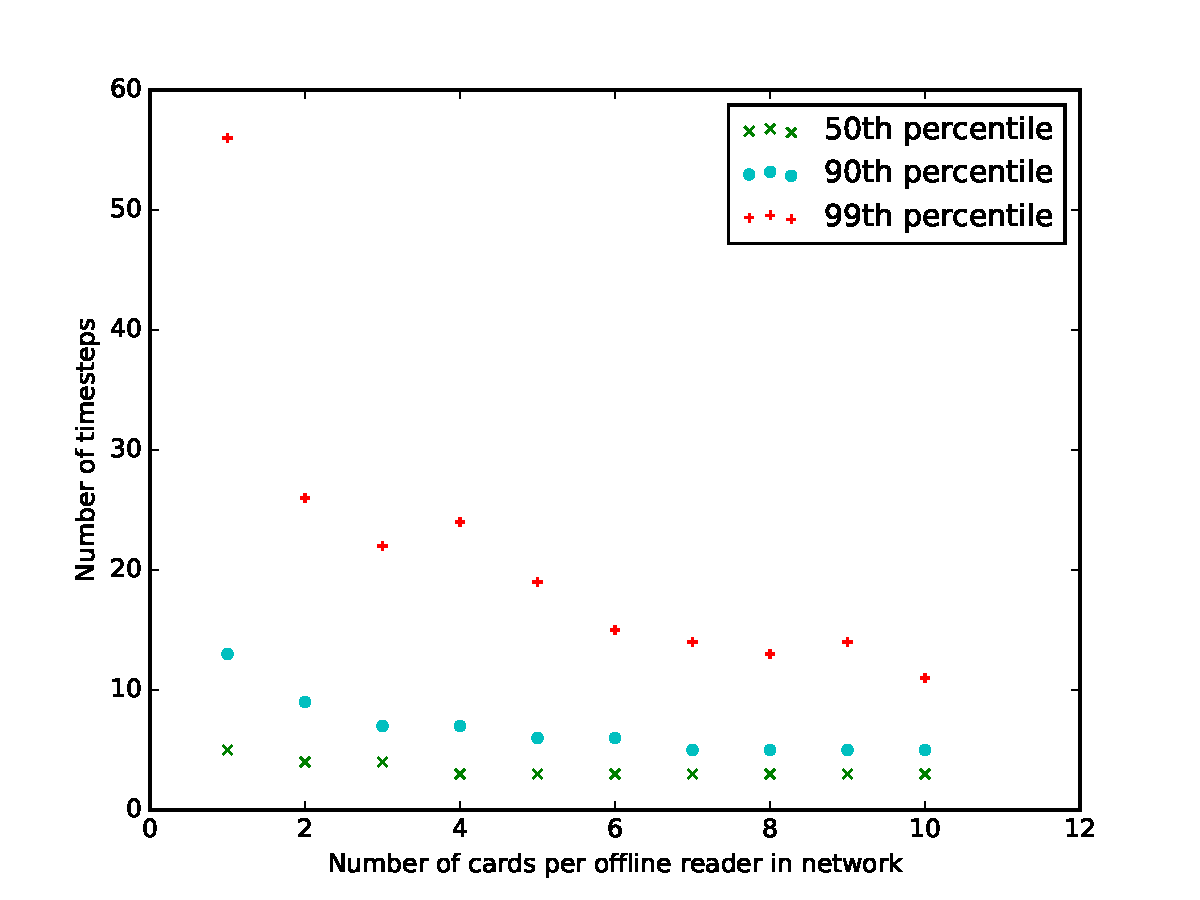
\includegraphics[width=\linewidth]{single_card_500_time.pdf}
    \caption{Timesteps to update readers with revoked UID (\SI{500}{readers})}\label{fig:sim_single_500_time}
  \end{figure}

  I'll reiterate that the absence of a link between a simulation timestep and a unit of actual time is intentional. The simulations can, within the assumptions of the model, determine how many taps and timsteps are required on each reader before the UID is propagated to it. They cannot determine how long this will take without making assumptions about how frequently cards are used. Any such assumption would be accurate for only a few networks, as the frequency with which cards are used can vary greatly between different card deployments. Within some deployments each card is used several times a day, where as in others a significant proportion of the cards may be dormant for months at a time.

  \begin{figure}[p]
    \centering
    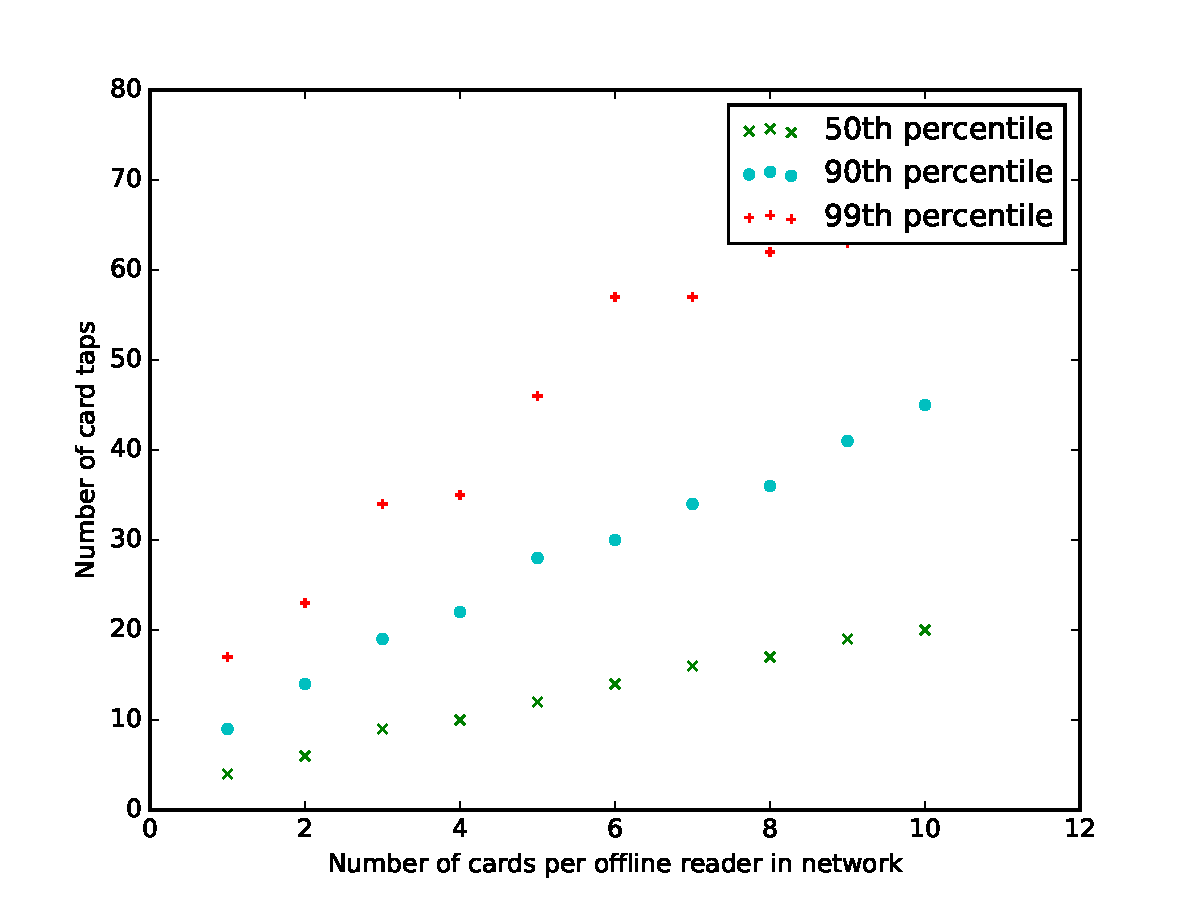
\includegraphics[width=0.58\linewidth]{single_card_100.pdf}
    \caption{Card taps to propagate UID (100 offline and 10 online readers)}\label{fig:sim_single_100}
  \end{figure}
  \begin{figure}[p]
    \centering
    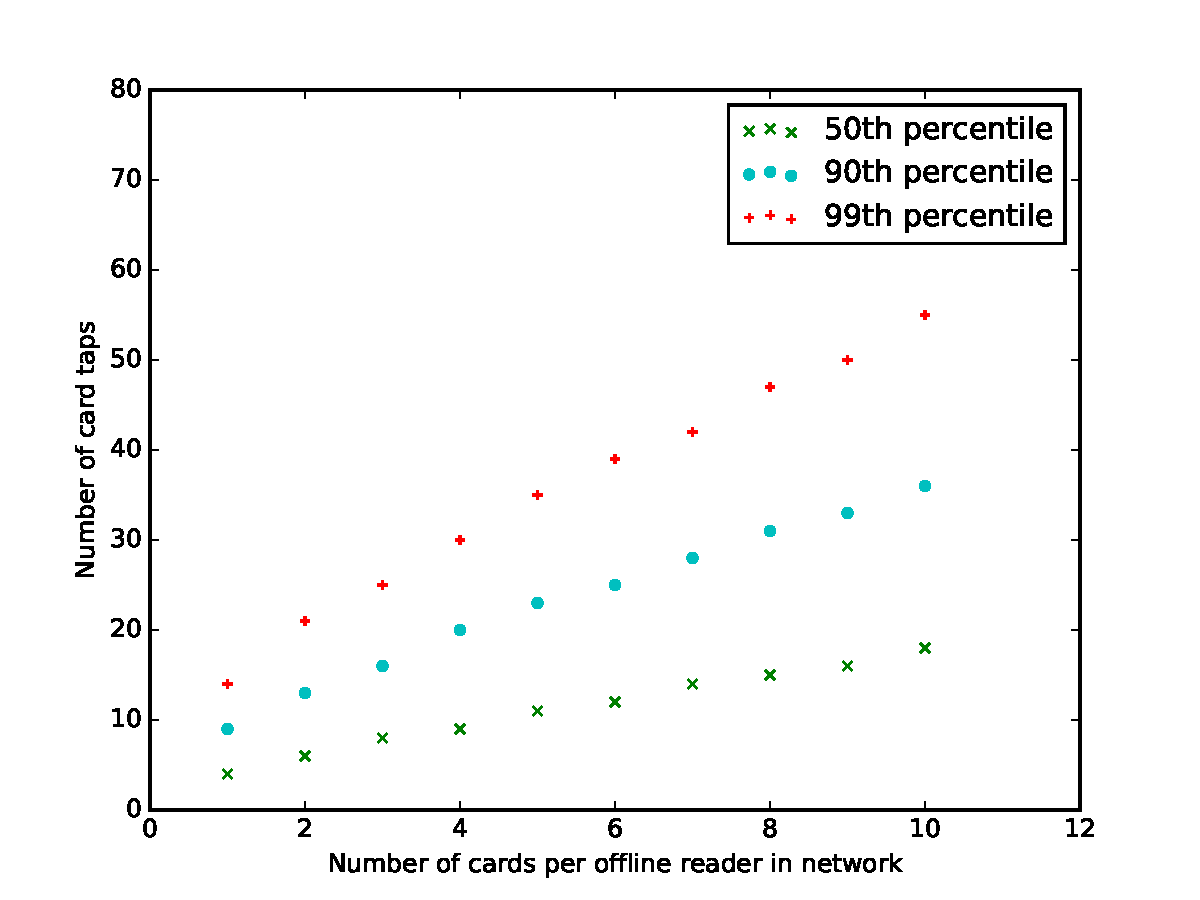
\includegraphics[width=0.6\linewidth]{single_card_1000.pdf}
    \caption{Card taps to propagate UID (1000 offline and 100 online readers)}\label{fig:sim_single_1000}
  \end{figure}
  \begin{figure}[p]
    \centering
    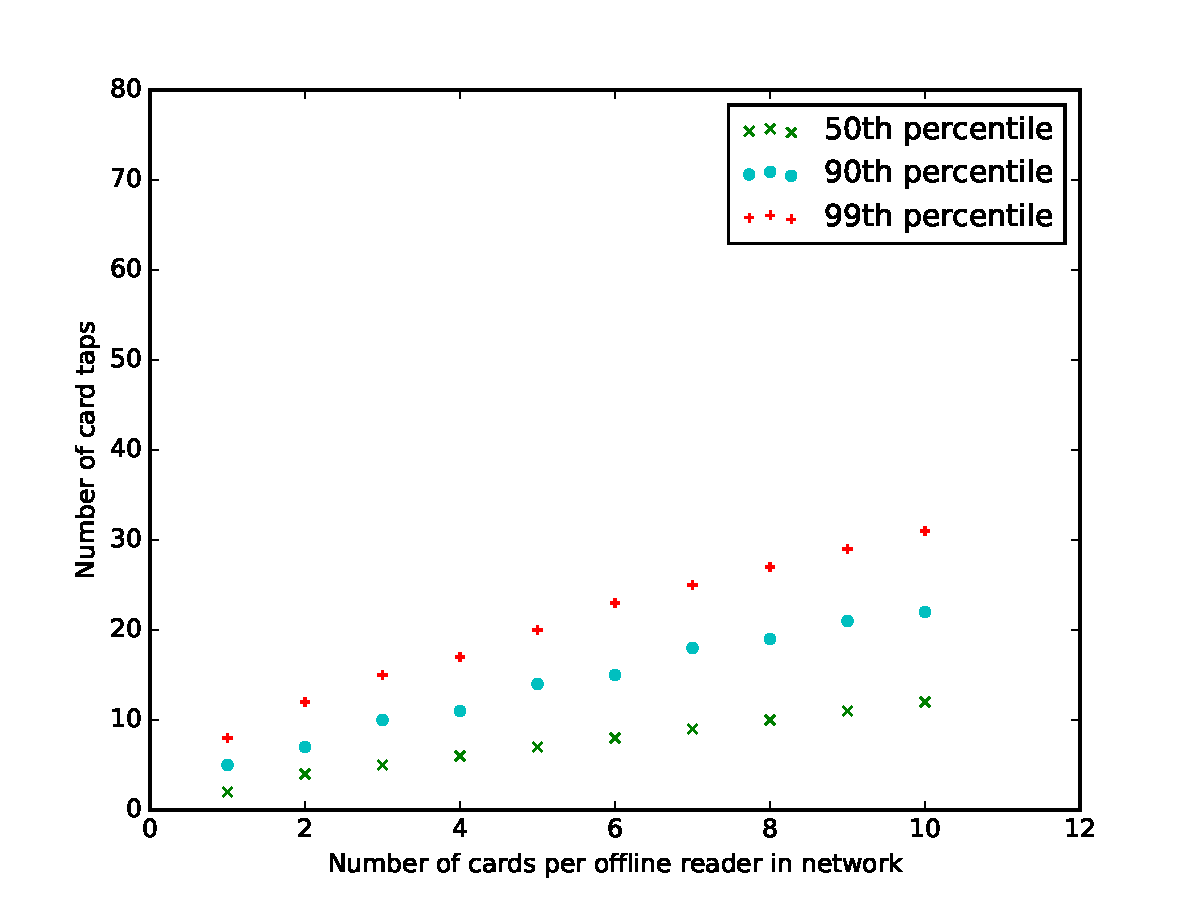
\includegraphics[width=0.6\linewidth]{single_card_500_online.pdf}
    \caption{Card taps to propagate UID (500 offline and 500 online readers)}\label{fig:sim_single_500_online}
  \end{figure}

  Both Figure~\ref{fig:sim_single_500} and Figure~\ref{fig:sim_single_500_time} used a network with 500 readers. Simulations using 100 and 1000 readers produced similar results as shown in Figures~\ref{fig:sim_single_100} and~\ref{fig:sim_single_1000}. As expected, increasing the number of online readers improves performance as shown in Figure~\vref{fig:sim_single_500_online}.

  \subsection{Revoking several cards at once}

  If the number of revoked UIDs is less than the capacity of the revocation sector (12 UIDs) then each algorithm can simply place all revoked UIDs into the revocation sector. As previously mentioned, this gives a good indicator of the inherent difficulty of a network but does little to stress test each algorithm. If the number of revoked UIDs exceeds the capacity of the revocation sector, then the algorithm must choose a subset of the UIDs to place in the sector.

  In this subsection I evaluate how well the na\"{\i}ve and random algorithms perform when several UIDs are revoked at once. The simulations use a network of 500 offline readers, 50 online readers, and 500 cards. For each timestep, the simulation records the percentage of propagations that have occurred. A propagation occurs when an offline reader sees a revoked UID for the first time and updates its internal list.

  Figure~\vref{fig:crowd_13} shows the relative performance of both the na\"{\i}ve algorithm and the random algorithm when thirteen UIDs (one more than the capacity of the revocation sector) are revoked at once. As is evident from the graph, the na\"{\i}ve algorithm completely fails to propagate one of the UIDs.

  \begin{figure}[h]
    \centering
    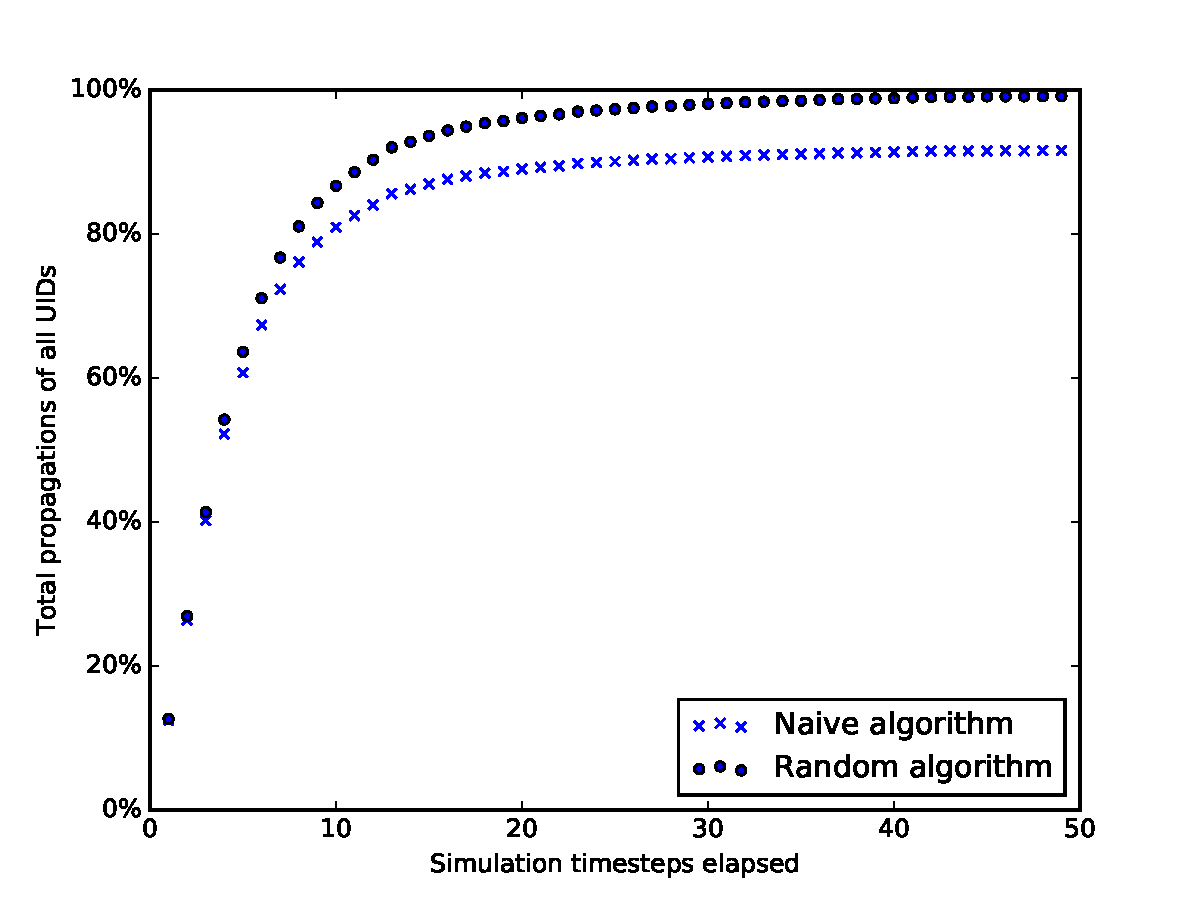
\includegraphics[width=0.9\linewidth]{crowd_500_13.pdf}
    \caption{Propagation of 13 UIDs}\label{fig:crowd_13}
  \end{figure}

  The performance improvement of the random algorithm over the na\"{\i}ve algorithm increases as the number of revoked UIDs increases. Figure~\vref{fig:crowd_24_60} shows the performance with 24 and 60 UIDs (2 and 5 times the revocation sector capacity respectively). From Figure~\vref{fig:crowd_60} it can be seen that the performance remains reasonable even when more than $10\%$ of the total cards are revoked at once.

  \begin{figure}[h]
  \centering
  \begin{subfigure}{.5\textwidth}
    \centering
    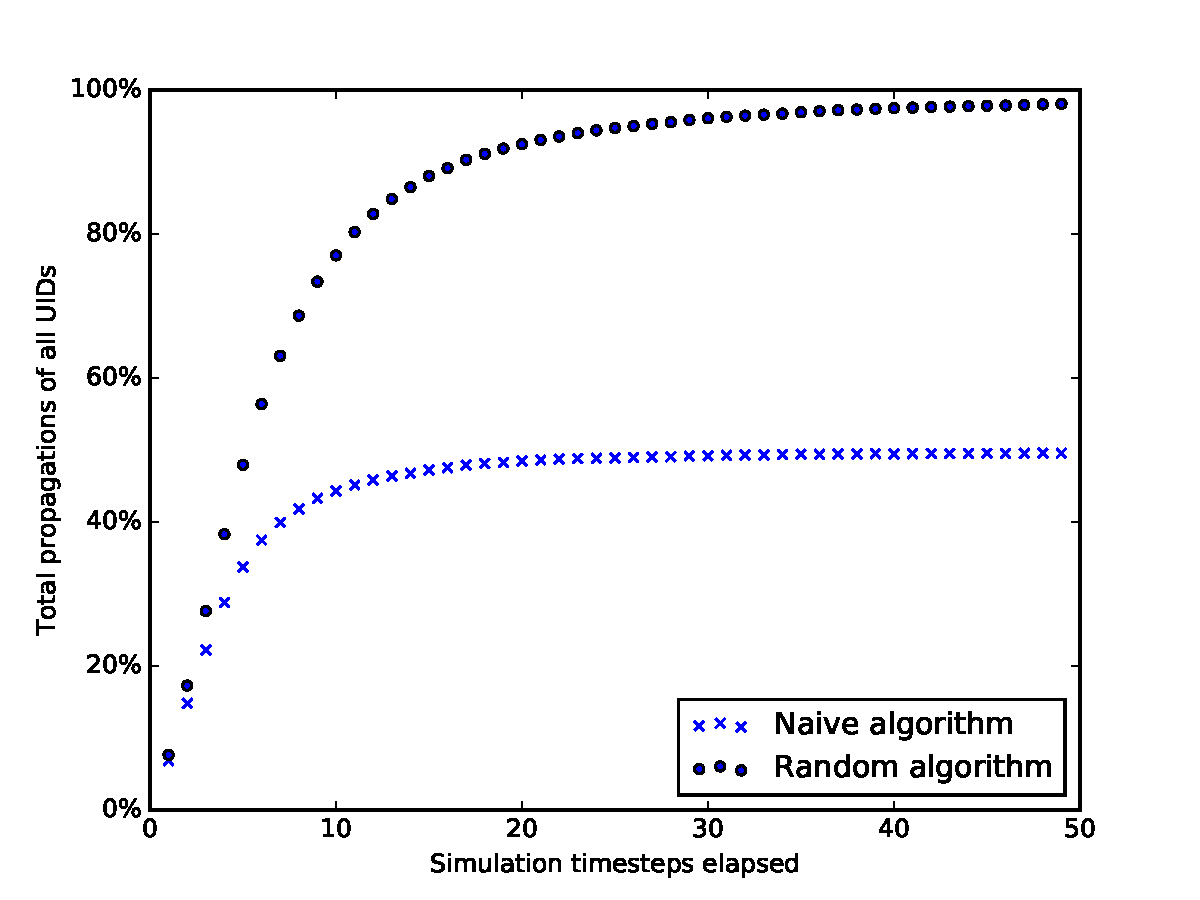
\includegraphics[width=\linewidth]{crowd_500_24.pdf}
    \caption{Propagation of 24 UIDs}\label{fig:crowd_24}
  \end{subfigure}%
  \begin{subfigure}{.5\textwidth}
    \centering
    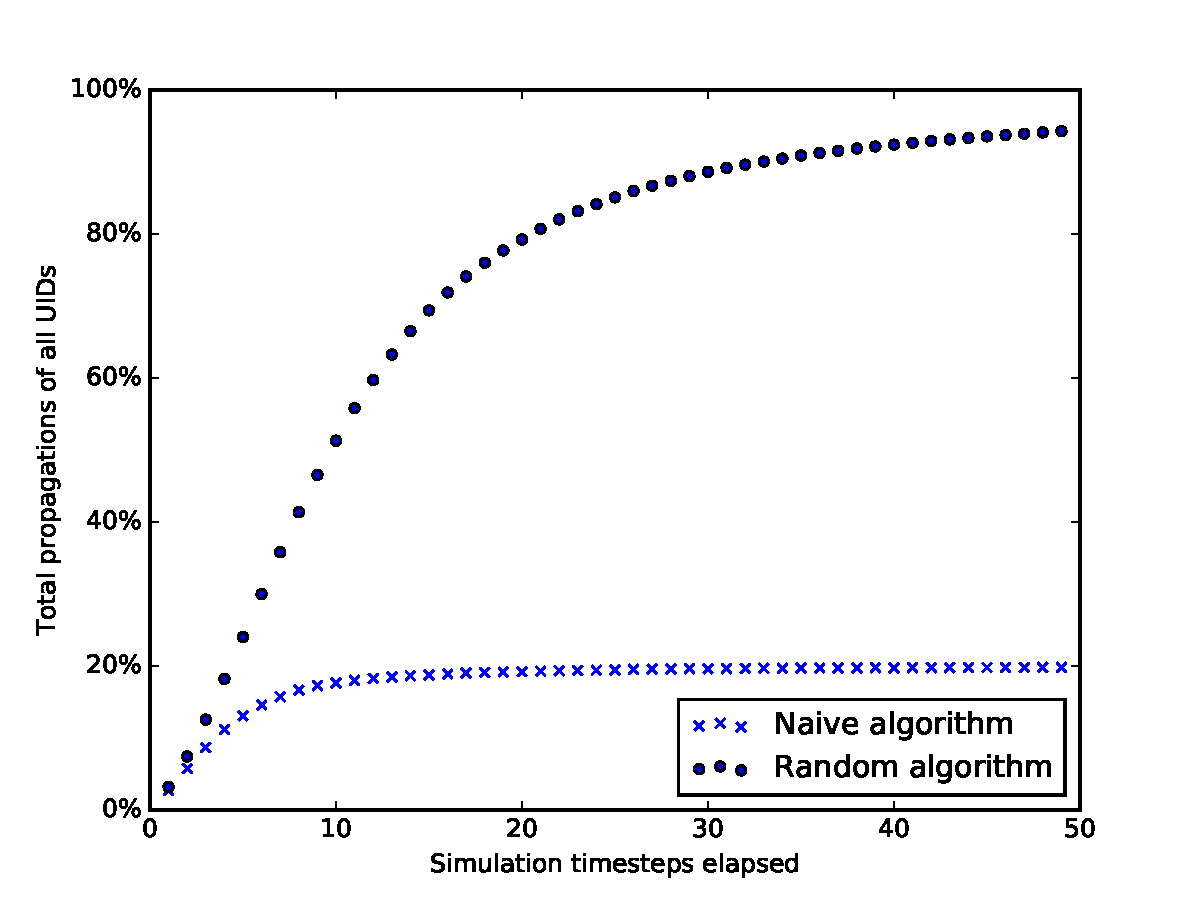
\includegraphics[width=\linewidth]{crowd_500_60.pdf}
    \caption{Propagation of 60 UIDs}\label{fig:crowd_60}
  \end{subfigure}
  \caption{Performance with varying numbers of UIDs}\label{fig:crowd_24_60}
  \end{figure}


  \subsection{Increasing number of revoked cards}

  The total number of revoked UIDs increases over time. The random algorithm selects UIDs at random, irrespective of how long ago they were revoked. Over time, the proportion of all revoked UIDs that have been recently revoked decreases, and thus the recently revoked UIDs are placed on cards with decreasing frequency. The performance of the random algorithm, therefore, decreases as the total number of revoked cards increases.

  As described in Section~\ref{sec:skewed}, the skewed random algorithm accounts for this by weighting the UIDs to ensure that recently revoked UIDs take precedent over those that have already been propagated. Figure~\vref{fig:chain_1000_100_25} shows how well each algorithm propagates $25$ UIDs with $100$ existing revoked and fully propagated UIDs. Increasing the number of revoked UIDs has little effect on the skewed algorithm, as shown in Figure~\ref{fig:chain_1000}. As shown in Figure~\ref{fig:chain_1000}, increasing the number of revoked UIDs has a huge impact on the performance of the random algorithm but almost no impact on the skewed algorithm.

  \begin{figure}[p]
    \centering
    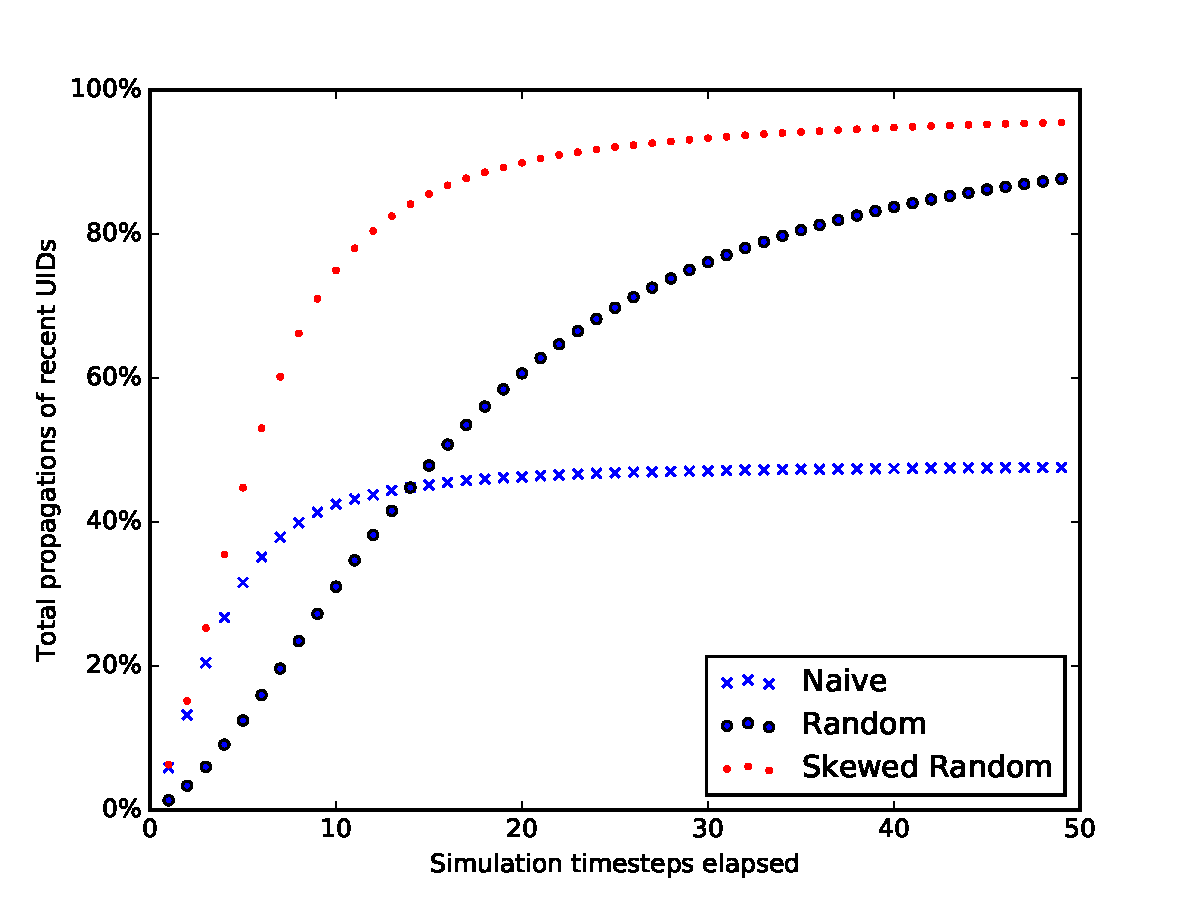
\includegraphics[width=\linewidth]{chain_1000_100_25.pdf}
    \caption{Propagation of 25 new UIDs with 100 fully propagated UIDs}\label{fig:chain_1000_100_25}
  \end{figure}


  \begin{figure}[p]
  \centering
  \begin{subfigure}{.5\textwidth}
    \centering
    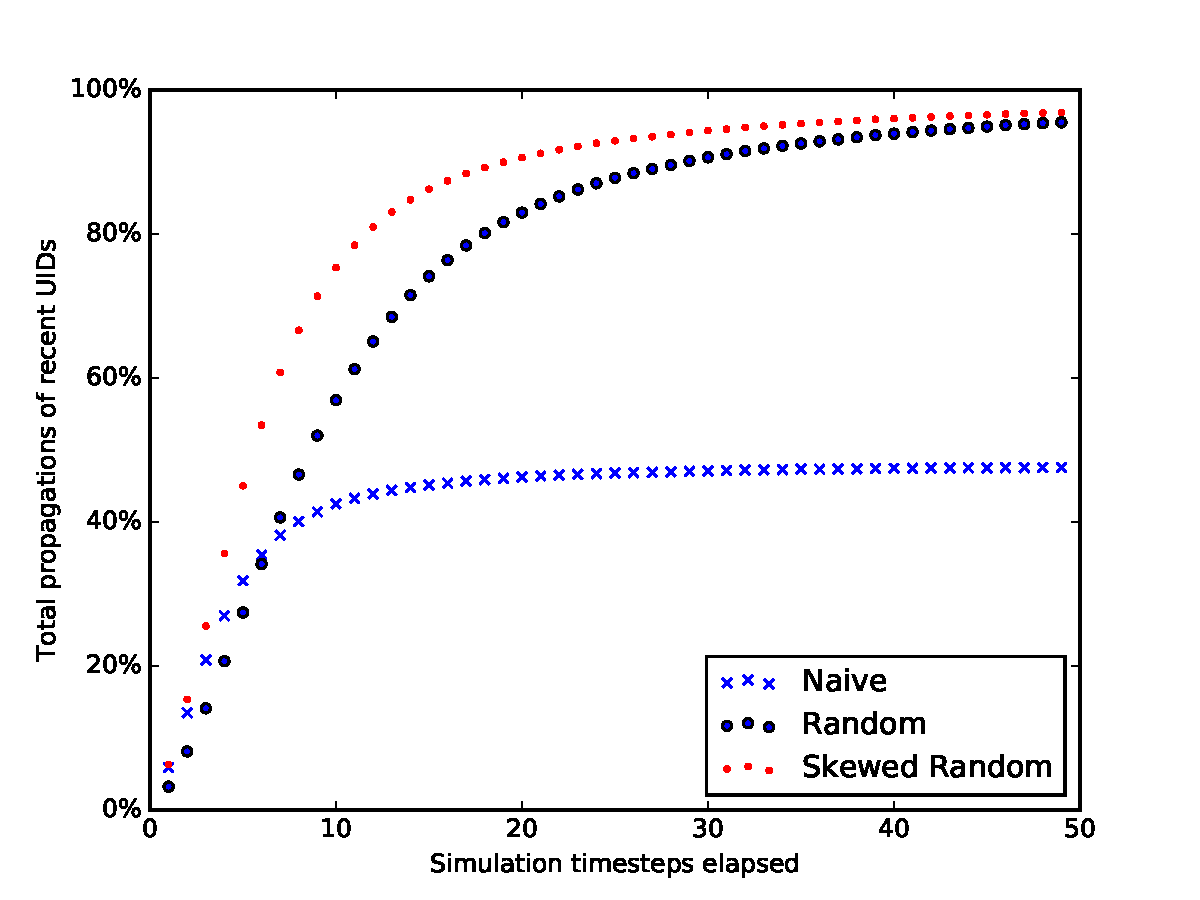
\includegraphics[width=\linewidth]{chain_1000_25_25.pdf}
    \caption{Performance with 25 existing UIDs}\label{fig:chain_1000_25_25}
  \end{subfigure}%
  \begin{subfigure}{.5\textwidth}
    \centering
    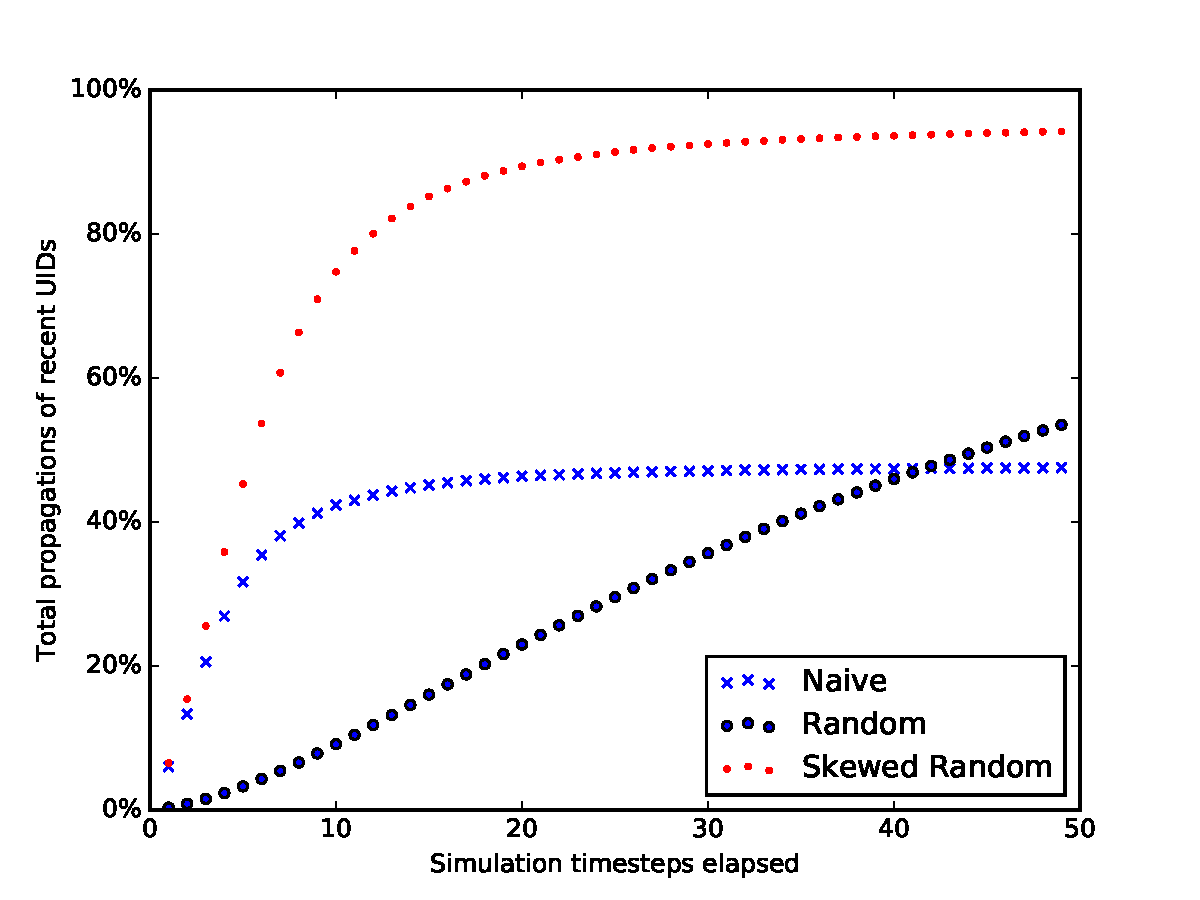
\includegraphics[width=\linewidth]{chain_1000_500_25.pdf}
    \caption{Performance with 500 existing UIDs}\label{fig:chain_1000_500_25}
  \end{subfigure}%
  \caption{Performance with varying numbers of fully propagated UIDs}\label{fig:chain_1000}
  \end{figure}

  \pagebreak

  \section{Simulation Suite}

  The simulation suite was instrumental to the success of the gossip protocol. Without the ability to simulate arbitrary networks, I wouldn't have had the data required to guide the changes (such as skewing). In this section, I evaluate the decisions I made and the performance of the simulation suite.

  The simulation suite was wrapped in a command line application to make it easy to simulate different network configurations. The output of the CLI (as shown in Figure~\ref{fig:chain}) contains all of the configuration values in the header. This allowed me to pipe the simulation output directly into a python script that generated appropriate graphs.

  \begin{figure}[h]
    \begin{code}[numbers=none]{{}}
      $ chain -offline=10 -alreadyRevoked=0 -newlyRevoked=1 -samples=2 -timesteps=5
      # chain: 2, 5, 10, 0.100000, 1.000000, 0, 1
      # sample: 0, rndSeed: 10
      0: 0, 0, 0
      1: 1, 1, 1
      2: 2, 2, 2
      3: 4, 4, 4
      4: 7, 7, 7
      # sample: 1, rndSeed: 11
      0: 0, 0, 0
      1: 1, 1, 1
      2: 2, 2, 2
      3: 3, 3, 3
      4: 4, 4, 4
      $
    \end{code}
    \caption{Output from simulation suite}\label{fig:chain}
  \end{figure}


  \subsection{Choice of language}

  When benchmarking the performance of each algorithm, the simulation is run on 10 different semi-randomised networks to ensure that the results are not specific to a single network. The extensive concurrency support that the Go programming language provides has been useful for optimising the performance of the simulation suite. Go's goroutines makes it easy to run these simulations in parallel, making full use of all the CPU cores available.


  \subsection{Performance}

  Several optimisations were made to improve the performance of the simulation suite. The mock driver in my \mifare{} library contains a software implementation of all the \mifare{} Classic card logic. After using the Go profiler it became apparent that the majority of the running time was spent carrying out these operations rather than doing the actual simulation. To reduce the running time, I implemented a fake driver that only supported reading and writing the revocation sector, and did not do any access condition verification. The fake driver reduced the running time by a factor of five.

  The running time is of order $\mathcal{O}(x \times y)$ where $x$ is the number of simulation timesteps and $y$ is the number of cards. Since each timestep involves moving each card to a new reader, the order cannot be reduced. Each timestep of the simulation has two parts; the first part moves each card and taps it on the new reader, the second part then queries each reader to collect the simulation metrics for that timestep.



  %\subsection{Simulation accuracy}

  %the simulation suite aims to provide an accurate model of a real-world network of readers. It's not possible, without real-world data, to definitively assess how well the simulation suite corresponds to reality.


\end{document}
